\chapter{DEFINING SYSTEM-LEVEL PROPERTIES}
\thispagestyle{plain}

\label{Defining}

% Definition of a system-level property
System-level properties play a central role in this dissertation.
A system-level property is a mathematical measurement of some non-explicit concept of interest in a agent-based model.
These properties are typically non-explicit, which means that inferring their values from just the given agent-level configuration parameters is difficult.

% Discuss how system-level properties are identified
% Discuss how system-level properties are mathematically defined
Identifying which system-level properties of an ABM to analyze is the first step of using the \framework.
Deciding on which features to be measured is a task for the user of the framework and will be influenced by what that user finds interesting or what that user needs to analyzed.
Each system-level parameter is defined as a mathematical measurement of the behavior in terms of observable features of the ABM.
For example, the average number of sheep in the Wolf Sheep Predation model is a system-level property of the system that is calculated by averaging the number of sheep measured in each time step over the lifetime of the system.
The framework utilizes the user provided mathematical definition to create a data set that is used in the forward mapping.

% Give an outline of the chapter
In this chapter, I discuss the problem of defining system-level properties for use in \fw.
First, the important ``stability assumption" and the consequences of this assumption are explained.
Next, a comprehensive list of common system-level property classes are outlined.
This list should be useful for users of \fw in defining their own system-level properties.
Then, the process in which \fw uses to sample an ABM is explained.
Finally, software implementation details are given for this particular step of \fw.


\section{The Stability Assumption}

% Before delving into the topic of defining system-level properties, I first discuss this assumption
Before delving into the topic of defining system-level properties, I first discuss the ``stability assumption."
Understanding this assumption and its consequences is important in defining system-level properties so that they will be measured accurately by \fw.

% A measurement of a system-level property should be stable.
% Explain what stable means
%  the sampling error is normally distributed 
% For example, the percentage of trees burned down
\fw assumes that the naturally occurring error for sampled values of a system-level property must have the following feature: the expected mean and expected median of the behaviors should be identical.
In other words, the errors should be expected to be evenly distributed around some value $\bar y$, in  both magnitude and quantity.
Errors following a normal distribution will have this property.
For example, the percentage of trees burned down in the Fires\footnote{More on the Fires model is discussed in Section \ref{sec:Fires}} model will vary from run to run, but for the most part will be centered around one value for a particular configuration.

% Explain the need for stability - we are trying to develop a functional mapping to solve the forward-mapping problem. Without this assumption, we cannot use regression(see background).
This assumption is important because if this assumption does not hold, regression algorithms will converge to predict with bias.
As more points are sampled, the regression algorithm predictions will converge on the value provided by the mean of measured values.
However, the median may be a better predictor of the expected behavior if the errors are not normally distributed.
This problem is best explained with an example.

A good example of 

% This is an example explaining the need for stability
In the Wolf Sheep Predation domain, a simple system-level measurement is the average number of wolves after a thousand time steps.
This number can be misleading, because certain configurations will \textit{sometimes} result in the wolves going extinct (i.e., zero wolves).
Other times, the same configurations will result in the wolves converging to a stable non-zero population.
When the wolf population does stabilize, it converges upon generally the same population value, $\bar w$.
However, the average of successive runs will result in a biased value between zero and this stable population size.
Unfortunately, this average is not useful in any way, since it does not tell how often the wolves will go extinct or what their population will be, should it be the case that the population stabilizes.

%% Have a figure here that shows a histogram of wolf populations given the same configuration.
%% It will show a large number of wolf populations at zero and then a bell-curve like structure near the true value.
%% Show the median and the mean

To remedy this problem, the average can be decomposed into two components: the case of going extinct and the case of not.
The average number of wolves $\bar w$ can be decomposed as:
\[\bar w = \mathrm{P}(extinct) * (\bar w | extinct) + (1 - \mathrm{P}(extinct)) * (\bar w | \neg extinct) \]
where $extinct$ is true when the wolves went extinct, $\mathrm{P}(extinct)$ is the probability wolves go extinct, and $(\bar w | \neg extinct)$ is the average number of wolves, given they did not go extinct.
The value of $(\bar w | extinct)$ is zero, so the left hand side of the above equation is zero.
Therefore, the equation can be simplified to:
\[\bar w = (1 - \mathrm{P}(extinct)) * (\bar w | \neg extinct) \]

As stated earlier, $\bar w$ is biased because sometimes an experiment with return zero and sometimes it will return $(\bar w | \neg extinct)$.
However, the values $\mathrm{P}(extinct)$ and $(\bar  w | \neg extinct)$ are useful in describing the system's behavior and are more stable (and accurate) than just using $\bar w$.
The system-level properties that should be measured for the Wolf Sheep Predation model is not the average number of wolves, but the average number of wolves given that they did not go extinct, and the probability of the wolves going extinct.

To calculate the value of $\mathrm{P}(extinct)$, divide the number of samples that exhibited zero wolves by the number of total samples for that configuration.
To calculate the value of $(\bar w | \neg extinct)$, average the population size of the wolves, only in samples in which they did not go extinct.

The histogram in Figure \ref{fig:num_wolves} illustrates why $\bar w$ is a poor metric for this domain.
I measured the average number of wolves post-convergence in 850 runs of the same configuration\footnote{grass-regrowth-time = 22, initial-number-sheep = 100, initial-number-wolves = 50, \\
sheep-gain-from-food = 4.7, wolf-gain-from-food = 20, sheep-reproduce = 3\%, wolf-reproduce = 4\% } of the Wolf Sheep Predation model.
In this experiment, 303 of the 850 samples resulted in wolves going extinct.
The other 547 samples had their wolf populations stabilize.
The average number of wolves over all samples $\bar w$ is 44.69.
The value 44.69 has little meaning in this domain, as it does not tell us about the stable wolf population size, or how often the system will exhibit zero wolves.
The estimated probability of extinction is $P(extinct) \approx 303 / 850 \approx .356$.
The average number of wolves in a stable population is $(\bar w | \neg extinct) = \sum (w_i) / 547 \approx 69.45$.
These two values explain the the behavior of this particular Wolf Sheep Predation model instance better than $\bar w$.

\begin{figure}[ht]
\centering
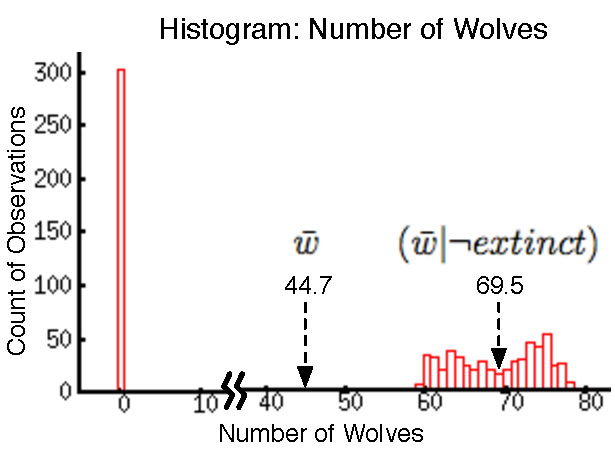
\includegraphics{images/num_wolves.pdf}
\caption{A histogram of the number of wolves after many successive runs shows that the average number of wolves is a poor number to use to describe the behavior.}
\label{fig:num_wolves}
\end{figure}


% In most situations, a nonstable measurement could be the result of two situations: there is an underlying threshold effect or biased readings before convergence.
In most situations, non-stable system-level properties are the result of some sort of \textit{threshold effect}.
Threshold effects are sudden changes in behavior, given a small change in the configuration.
Threshold effects are also sometimes referred to as \textit{tipping points}.
In ABMs that incorporate random behavior, configurations that lay on a boundary of a threshold effect can exhibit erratic behavior, which was the case with the Wolf Sheep Predation example.
Typically, this problem can be overcome by decomposing the property into several sub-properties that describe the threshold effect. 
This approach is what was needed to provide useful and accurate information in the Wolf Sheep Predation example.

\section{Common Classes of System-Level Properties}

% Many system-level properties can fit into a certain category
Through the course of identifying a number of system-level properties in a variety of domains, I have found that most properties fit into one of these general classes.


\subsection{Average of a Value}
% average value over the life of a system
One of the simplest measurements is the average value of a property over the life of the system.
This is useful for measuring behavior that converges over time.
To measure this property, the property is measured every time step up until a predetermined stopping point, and then averaged.

\begin{figure}[ht]
\centering
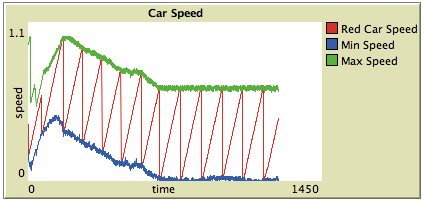
\includegraphics[scale=.75]{images/traffic_converge.png}
\caption{The behavior of the NetLogo Traffic Basic ABM converging after about 650 time steps.}
\label{fig:traffic_converge}
\end{figure}


A few modifications to this simple approach are possible.
First, the recording of values can be ignored for a number of time steps to allow the system to converge.
If convergence is ignored, the values recorded before convergence may bias the results in an unexpected way.
To remedy this, only the points post-convergence are used for the average.
The next step is to determine what this ``post-convergence" happens.
The simplest method is to determine a duration of time in which most model will have converged.
Another naive method is to just sample for a very long time.
As time passes, the average will converge to the convergent value, since more values representing the convergent behavior will factor into the average.
A more advanced technique would be to detect when the system values have stopped drastically changing and start measuring from there.

In Figure \ref{fig:traffic_converge} (a plot from the NetLogo Traffic Basic ABM), the maximum speed and minimum speed of the vehicles converge to .65 and 0, respectively.
However, before time step 650, the behavior was quite different than the eventual convergent behavior.
If each time step (0 to 1250) were averaged, the value would be biased to be larger than .65.
This number has meaning, but not the ``average top speed" that was expected.
The average should be comprised of values after time step 650 to match the actual measurement with the expectations.

This class of measurement should not be used on properties that diverge (i.e., fail to converge on a single value over time).
In divergent cases, the average will continue to increase or decrease as more time steps are used in the measurement.
However, it should be the case that the average value converges as more time steps are measured.
The value produced by the forward and reverse mappings will be inaccurate and meaningless if this property does not hold.
This is because the value would be dependent on how many time steps the system was sampled, and would have very little to do with the value of the behavior itself.

\subsection{Variance of a Value}
% variance of a value over the life of a system
The variance of a value over the life of a system is a useful metric for determining how ``stable" the behavior is.
If the behavior changes wildly from time step to time step, the variance will be relatively high to one in which the value remains stable.
See Figure \ref{fig:variance_compare} for a comparison between two situations in which the variance of values are different.

\begin{figure}[ht]
\centering
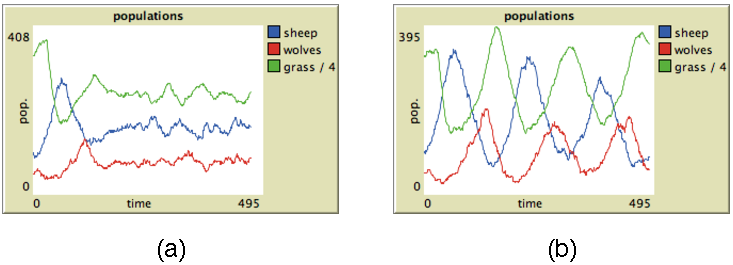
\includegraphics{images/variance_comparison.pdf}
\caption{Two different behaviors in the NetLogo Wolf Sheep Predation ABM with similar average sheep, wolves and grass values. The two can be distinguished by the variance: the values in (a) have a lower variance than the ones in (b).}
\label{fig:variance_compare}
\end{figure}

Similar to averaging system-level properties over time, only values after convergence should be used to calculate the variance.
This must be done to avoid biasing the variance of the behavior after it has converged.
Taking this problem into consideration is particularly important in this for the variance metric because systems' behaviors typically vary significantly before convergence.

Also similar to the average value metric, this variance metric should not be used on behaviors that diverge.
As a divergent property value continues to increase or decrease, the variance will increase.
The variance should converge on a single value as more time steps are sampled, for the same reasons that the average metric should converge.


\subsection{Probability of a Threshold Effect}
% probability of an event occurring in the system
Threshold effects are binary properties that may or may not happen in a system.
These tipping points divide the behavior space into configurations that exhibit the threshold effect and ones that do not.
Configurations near the threshold will often times vary between which behavior side of the threshold it will converge on, run after run.
For example, in the Wolf Sheep Predation ABM, wolves may or may not go extinct while the system is approaching convergence.
With some configurations, the wolves will always go extinct, but in others the wolves never go extinct.
Configurations on the boundary between wolves going extinct and not will exhibit both of these in different runs due to the inherent randomness in the system.

One particularly useful metric for analyzing threshold effects is the probability that a certain configuration will exhibit the threshold effect.
For example, in the Wolf Sheep Predation ABM, a percentage could represent the probability that the configuration will result in the wolves going extinct.
To measure this property, several experiments need to be executed for a single configuration. 
The probability is estimated by calculating the proportion of iterations that had no wolves, to the total number of experiments.
The value of this probability should converge as more experiments for a single configuration are executed.




\subsection{Measuring a Value That Changes Over Time}
The previous measurements assume that the behavior will converge over time.
Also, there are situation in which the average value or the variance of a value does not convey enough information.
% There are a number of properties that change over time  want to be measured
There are properties that change over time that do not fit into the above classes.

% So far, all properties have had scalar values,
So far, all properties have been scalar values.
The framework works only with scalar values and is unable to naturally predict how a behavior will change over time.
% therefore, it may seem that it is impossible to measure behaviors over time, since these properties change.
% With a change of perspective, this is possible.
% to measure a system-level behavior that changes over time, the system-level properties used by \fw are scalars that represent this behavior in a parametric model.
To circumvent this issue, the system-level properties could be parameters of a parametric model that represents a behavior that changes over time.
This is essentially a nonlinear regression problem, in which the independent variable is time and the dependent variable is the property.

% The parameters are the system-level properties are learned in the forward mapping process and can be used to predict the parameters of the model.
The parameters of the behavior's parametric model are learned in the forward mapping process as individual prediction problems.
$N$ different forward mappings will be learned for each $N$ parameter.
The value for each parameter is predicted with each mapping, given the configuration.
These parameters are plugged into the parametric model to generate a curve that represents the behavior over time.

\begin{figure}[ht]
\centering
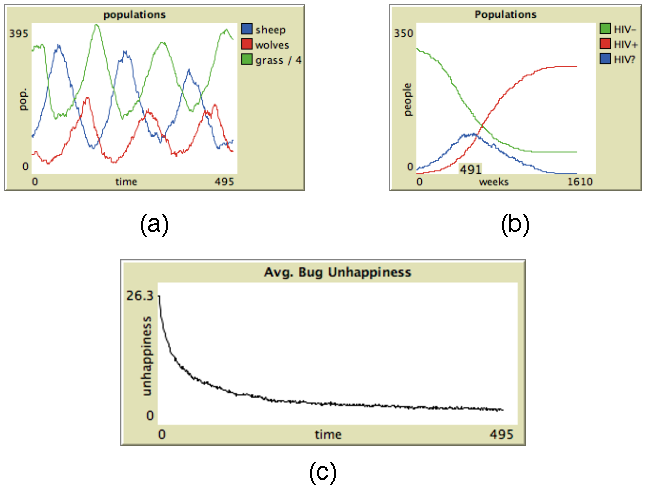
\includegraphics{images/overtime_compare.pdf}
\caption{Different types of behaviors that change over time in NetLogo ABMs. }
\label{fig:overtime_compare}
\end{figure}


This approach can be applied to a number of phenomena, such as the ones illustrated in Figure \ref{fig:overtime_compare}.
In \textit{(a)}, the values of animal populations in the Wolf Sheep Predation model vary rhythmically and could modeled with sine curves.
The parameters of these behaviors modify the magnitude, height and frequency of the sine curves.
In \textit{(b)} (a plot from the NetLogo AIDS model \cite{aids}), the \textit{HIV-} (people without HIV) curve decreases and the \textit{HIV+} increases with following a sigmoid.
The parameters of these two sigmoid behaviors modify the shape of the sigmoid.
The \textit{HIV?} (people that have HIV but do not know it) value appears to follow a curve that is similar to a probability distribution. 
However, it is simpler to model this property in terms of the other two: the HIV- and HIV+ values subtracted from the total population.
In \textit{(c)} (a plot from the NetLogo Firebugs model \cite{bugs}), the behavior converges to zero over time.
The rate of convergence (i.e., the slope of the curve) would be the parameter for the model of this behavior.
This general approach is applicable to any property that can be described by a parametric regression model.

These system parameters are measured during sampling by performing parametric nonlinear regression for each experiment
to determine good values of the parameters.
These parameters are the system-level properties for \fw, but can be interpreted by the user as the parameters to the regression model.

Custom models can be developed for particular domains.
Consider the NetLogo Traffic Simple simulation, in which cars move in a single lane.
Traffic jams appear in waves, which is illustrated by the movement of the red car in Figure \ref{fig:traffic_converge}.
We would like to develop a mapping to represent the velocity of the red car.
From visual observation, it appears that the red car has a constant minimum speed and a maximum speed.
It is known that the acceleration is linear from the programming of the model.
Also, the red car follows a rhythmic behavior: the car reaches a certain speed, then stops.
 With these, all that is needed to create a wave-like parametric model that describes this behavior is available.
 The following variables are used in the parametric wave model:
\begin{itemize}
  \item Let $A$ be the amplitude of the wave (i.e., the maximum velocity minus the minimum velocity)
  \item Let $T$ be the period of the wave (i.e., the time between the occurrence of a maximum velocity and the occurrence of a minimum velocity)
  \item Let $h$ be the height of the wave (i.e., the minimum speed)
\end{itemize}
The behavior within each period is linear, so it can be described as a simple linear model:
   \[speed(t) = \displaystyle \frac{A}{T} ~{} t + h\]
Since this behavior is periodic, modulus $T$ is used to reset the behavior back to the minimum spread.
   \[speed(t) = \displaystyle \frac{A}{T} ~{} (t~{}\mathrm{mod}~{} T) + h \]
The forward-mapping problem would involve predicting values for $A, T,$ and $h$, given the configuration of the system.
For each experiment, nonlinear regression is used to find good values for $A, T,$ and $h$, which are recorded as the dependent variables.



\section{Sampling}
The sampling process may begin once system-level properties are defined.
% Two major steps:
%  1. Retrieve raw data from the simulation
%  2. Compute on that data to generate the properties of interest
The \fw sampling process consists of two major steps:
first, retrieve raw data (i.e., just simple property values at each time step) from the simulation, then, use that data to compute the values of the system-level properties (e.g., average and variance).
Instead of performing the calculations while sampling, I prefer a method of computing the actual statistics from a raw data set.
This way, new statistics could be measured using the raw data at a later point in time without having to re-sample the system.

% \fw typically uses a evenly distributed random sampling technique.
The \fw uses an evenly distributed random sampling technique.
Ranges for parameters are passed to the sampling program and random values within these ranges are generated for each experimental configuration.
%  this is useful for changing the size of the dataset dynamically
This technique is flexible because it allows me to change the size of the data set dynamically for testing purposes.
Also, new points can be sampled to increase the accuracy of the data set in a particular area.
The initial regression algorithms I have selected to work with \fw  work with randomly distributed data.
% More advanced sampling techniques could be used in the future.
More advanced sampling techniques could be used in future work.
See Subsection \ref{sec:fw_sampling} for a more in depth discussion of this possible extension to \fw.

% Sometimes... Discuss the need for doing several runs on the same configuration
Sampling the same point, instead of generating a new point per experiment, has several uses.
Different samplings of the same point could be used to:
\begin{itemize}
   \item Measure the variance of a variable between samples to determine its stability,
   \item Determine the probability of a threshold effect being exhibited,
   \item Smooth the data set by reducing natural error,
   \item Generate more accurate individual points, and more.
\end{itemize}
For these reasons, I suggest sampling each randomly selected point several times, instead of sampling a wider variety of points once.
% Discuss the selection of number of steps the ABM should run

\section{Implementation Details}

The \fw implementation for defining system-level properties and performing sampling is designed to require a minimal amount of user programming.
The sampling process consists of a number of distinct steps:
\begin{enumerate}
% Steps:
%  1. identify what properties are needed in the simulation and the ranges of values we want to configure --- that are needed to perform the system-level properties
\item Identify, by name, which NetLogo properties need to be extracted from the simulation in order to calculate the system-level properties;
Also, the user specifies how often (i.e., time steps passed) each property should be measured.
\item Specify all ABM configuration parameters by name, along with minimum and maximum values that random configurations will lie within;
%  2. Sample the ABM to generate a raw data set
\item Run the sampling application to generate the raw data set;
%  3. Pass the raw data set through a script that converts the raw entries into the desired system-level properties to create a new data set
\item Pass the raw data set through the map program, which converts the raw entries into a more compact data set that contains the desired system-level behaviors and relevant configuration parameters.
\end{enumerate}

% First step: the sampling program is written in java
%  the sampling program is given the ranges that are to be sampled,
%  and the data values that are needed
The sampling program is written in Java so that it can interface with NetLogo's Java API, which is used to run the ABMs.
All the user provided information is passed to this program in a text configuration file.
The details of this configuration file and how to write one is covered in Appendix \textit{[TODO]}.
A program which emits values with an identical format as the default sampling program could replace the default sampling program.
Replacing the default sampling program would be useful for taking more control of the sampling process, for instance to implement an advanced sampling strategy.

% The second step: the sampling program performs the sampling
The sampling program prints the raw data to standard out.
The data is tab delimited to separate items within entries and entries are delimited by newlines.
%  the raw data is returned to standard out. The data is tab delimited to separate items within entries. Entries are delimited by newlines.
Each entry is organized in the order specified in the configuration file, so the configuration file can be used to give the different columns identifiable names.
%  The output file could be redirected to a file to be stored for future use, if necessary
The standard out output could be redirected to store data in a file or piped to the next step.


% The third step: use the ``map" script to parse the raw data, and output a data set that contains the system-level properties.
In the final step of sampling, the ``map" Python program is used to parse the raw data and output a data set that contains the system-level properties.
%  the map script parses the data for each entry.
The map script parses the data for each entry.
%    the parse returned is a hash table object where the keys are the names of the raw data items and the values are the values inside, as strings.
The parse returns a hash table object (Python dictionary) per entry, in which the keys are the names of the raw data items and the keys are the values, as a string.
%  the map script is passed a user-created python module that is used to compute the values of the system-level properties, from the raw data.
The map script is passed a user-created Python module that is used to compute the values of the system-level properties from the raw data.
%  this user-created python module has a list of functions that each returns a value for a system-level property.
This user-created Python module contains a list of functions that each returns a value for a different system-level property.
%  map returns a new data set to standard out, containing the configuration parameters and the system-level properties.
Map returns new data sets to individual files (one per system-level property), containing the configuration parameters and the system-level property.
%  simple example
%  list example
%  More details on how to create this python module is covered in Appendix XX.
More details on how to create this Python module is covered in Appendix \textit{[TODO]}.
The name ``map" was chosen because it is a similar process to functional programming's \textit{map} function.

The output of the map function is then passed to the forward-mapping problem solver, which is covered in the next chapter.







